\documentclass[acmtog]{acmart}
\usepackage{graphicx}
\usepackage{subfigure}
\usepackage{listings}
\usepackage{color}

\definecolor{mygreen}{rgb}{0,0.6,0}
\definecolor{mygray}{rgb}{0.5,0.5,0.5}
\definecolor{mymauve}{rgb}{0.58,0,0.82}
\lstset{
 backgroundcolor=\color{lightgray}, 
 basicstyle = \footnotesize,       
 breakatwhitespace = false,        
 breaklines = true,                 
 captionpos = b,                    
 commentstyle = \color{mygreen}\bfseries,
 extendedchars = false,             
 frame =shadowbox, 
 framerule=0.5pt,
 keepspaces=true,
 keywordstyle=\color{blue}\bfseries, 
 language = C++,                     
 otherkeywords={string}, 
 numbers=left, 
 numbersep=5pt,
 numberstyle=\tiny\color{mygray},
 rulecolor=\color{black},         
 showspaces=false,  
 showstringspaces=false, 
 showtabs=false,    
 stepnumber=1,         
 stringstyle=\color{mymauve},        
 tabsize=2,          
 title=\lstname                      
}

% Title portion
\title{Assignment 1 : Creating your own OpenGL program} 
\author{Name:\quad Sun Weiliang  \\ student number:\quad 2020533010
	\\email:\quad sunwl1@shanghaitech.edu.cn}

% Document starts
\begin{document}
\maketitle

\vspace*{2 ex}

\section{Outline of the Assignment1}

In this assignment, we are taught to finish several tasks below:

1. Load Mesh from files

2. Phone Lighting

3. Camera control

Bonus part:

1. Play with light!

2. Geometry Shader

\section{The first task: Load Mesh from file}

\textbf{1.1 Load Mesh from file}

In this part of the assignment, we are provided with an object file. With some comments start with $\#$.

The first several lines are the coordinates of the vertices starting with $v$,containing a letter $v$ and three floats. Then comes several lines of the normal of the vertices starting with $n$,containing a letter $n$ and three floats. Finally, there exists several lines of face of the vertices starting with $f$, containing a letter $f$ and six ints.

First, to store the coordinates of the vertexes, I use a vector of vec3 named $vertex\_set$. To store the coordinates of the normals, I use a vector of vec3 named $normal\_set$.

By judgding the first char of the input string:

1. If it is $\#$, we choose to ignore it, then continue.

2. If it is $v$, we choose to store the following three floats into the $vertex\_set$.

3. If it is $n$, we choose to store the following three floats into the $normal\_set$.

4. If it is $f$, I create two new vectors named $vertex\_indices$ and $normal\_indices$ to store the final results in the vertices and indices. Because of the fact that I choose to use EBO, so I want to keep all the vertexes in the vertices unique to satisfy the EBO demand.

With the help of the temp vector, I totally succeed in storing the true vertices and indices into the vertice vector and indice vector. Also, testing code is like:

\begin{lstlisting}
	for(auto iter = bunny.vertices.begin();iter!=bunny.vertices.end();iter++)
    {
    	std::cout<<iter->position.x<<" "<<iter->position.y<<" "<<iter->position.z<<std::endl;
    }
    for(int i=0;i<bunny.indices.size();i++)
	{
     	std::cout<<bunny.indices[i]<<" ";
  	}
\end{lstlisting}

\textbf{1.2 Draw the mesh on the screen}

The second part of the first task is that we need to draw the mesh on the screen once it is exerted color. In this part we need the help of shader.

The init of the OpenGl can be briefly explained, we import three variables into the code:

1. Vertex Array Object named VAO

2. Vertex Buffer Object named VBO

3. Element Buffer Object named EBO

We need to create a VAO,VBO and EBO to handle the binding procedure. After binding we should import two shader language into the Class Shader, which are named $vertex\_shader.vs$ and $frag\_shader.fs$.(The geometry part will be mentioned in the following bonus part).

\textcolor[rgb]{1,0,0}{\textit{First part--vertex shader:}}

Layout location tells the procedure the location of the vertex attribute. And we also need to claim output which are named $world\_pos$ and $world\_normal$ to get the coordinates in the world space.

In this part we have three important matrixs which are: projection matrix, model matrix and view matrix. After using the three matrixs, we can get the object's world position and world normals in the world space, transmitting the local position and local normal to the world position and world normal. 

The model matrix transform the coordinates into the world space, and the view matrix transform the coordinates into the view space, and the final projection matrix projects the object into a cube.

The formula is as follows:

$$V_{clip}=M_{projection}\cdot M_{view} \cdot M_{model} \cdot V_{local}$$ 

Also we should define the projection matrix and view matrix, which is:

\begin{lstlisting}
	glm::mat4 view = glm::translate(view, glm::vec3(0.0f, 0.0f, -3.0f));
	glm::mat4 projection = glm::perspective(glm::radians(45.0f), Width / Height, 0.1f, 100.0f);
\end{lstlisting}

And then we can use uniform to put these two factors into the vertex shader. Also the function of setMat4() is essential for the transformation from $main.cpp$ to $vertex\_shader.vs$

\textcolor[rgb]{1,0,0}{\textit{Second part--fragment shader:}}

There is nothing special of the fragment shader in this part. More will be mentions in the following part phone lighting. In this part, the fragment shader only need to input the coordinates and output the color.

\clearpage

After the first part: loading meshes from file and draw the meshes on the screen, we get a bunny like the picture as follows:

\begin{figure}[h]
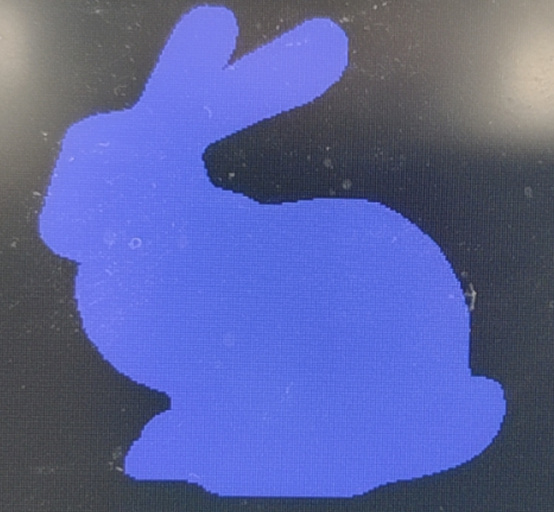
\includegraphics[width=4cm,height=4cm]{first_bunny}
\caption{the first edition of bunny}
\end{figure}

Obviously, the picture of the bunny is only a 3d model in the world space without any light exerted. In the next part, we will exert several light onto the surface of the bunny.

\section{The second task: Phone Lighting}

In this part, we need to exert phone lighting model which divides lighting into three distinct components: ambient, diffuse and specular. All of the three factors are computed separately and then added together.

Ambient lighting is a constant light model to simulate the world's normal light. The diffuse lighting will simulate the light's directional impact on the object, meaning that the more direct the object to the light, the lighter it will be. And the final specular light simulates some spot on the surface.

In this part, we will do more in fragment shader:

\textcolor[rgb]{1,0,0}{\textit{Setting ambient}}

This is nothing special, like the following code:

\begin{lstlisting}
	float ambient = 0.1;
	vec3 result_color = ambient*light_color*object_color;
	frag_color = vec4(result_color,1.0};
\end{lstlisting}

\textcolor[rgb]{1,0,0}{\textit{Setting diffuse}}

In this part we need to convey the normal from vertex shader to fragment shader. Also we need the light position of the light and the location of the fragment. The world position and world normal can be get from the vertex shader as the above report says.

The first thing we need to calculate is the direction vector between the light source and the fragment's position.The light's direction vector is the difference vector between the light's position vector and the fragment's position vector. So I normalize both the normal and the resulting direction vector:

\begin{lstlisting}
	vec3 normal_direction=normalize(normal);
    vec3 light_direction=normalize(light.position-world_pos); 
    float diffuse=max(dot(normal_direction,light_direction),0.0);
\end{lstlisting}

\textcolor[rgb]{1,0,0}{\textit{Setting specular}}

We negate the lightDir vector. The reflect function expects the first vector to point from the light source towards the fragment's position.We first calculate the dot product between the view direction and the reflect direction and then raise it to the power of 32. This 32 value is the shininess value of the highlight. The higher the shininess value of an object, the more it properly reflects the light instead of scattering it all around and thus the smaller the highlight becomes:

\begin{lstlisting}
	vec3 viewDir = normalize(viewPos - FragPos);
    vec3 reflectDir = reflect(-lightDir, norm);
    float spec = pow(max(dot(viewDir, reflectDir), 0.0), 32);
    vec3 specular = specular * spec * lightColor; 
\end{lstlisting}

And then add them together:

\begin{lstlisting}
	vec3 result = (ambient + diffuse + specular) * objectColor;
    FragColor = vec4(result, 1.0);
\end{lstlisting}

After this part, the bunny looks like: (the bunny has phone lighting)
\begin{figure}[h]
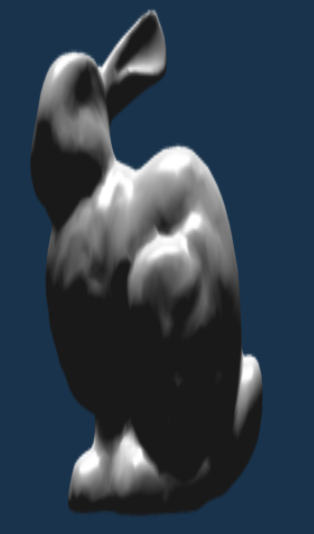
\includegraphics[width=4cm,height=4cm]{light_bunny}
\caption{the phone lighting of bunny}
\end{figure}

\section{ The third task: Camera control}

\textbf{3.1 Navigate in the virtual world}

Since we aren't provided the camera.h file, we can't use many operations in the .h file given by the completed part. So we ourselves create a camera point. The definition is as follows:

\begin{lstlisting}
	glm::vec3 initial(0, 0, 0);
	glm::vec3 front(0, 0, 1);
	glm::vec3 up(0, 1, 0);
	glm::vec3 right(1, 0, 0);
	glm::vec3 cam_front(0, 0, -1);
	glm::vec3 cam_right(-1, 0, 0);
	glm::vec3 cam_up(0, 1, 0);
\end{lstlisting}

And by using the glm lookat function, we change the origin view initial to the following:

\begin{lstlisting}
	View = glm::lookAt(cam_pos, cam_pos + cam_front, up);
\end{lstlisting}

After this, we can get the view in the virtual world by the camera.

\textbf{3.2 Walk around using keyboard input}

First we set the camera position to the previously defined cameraPos. The direction is the current position + the direction vector we just defined. This ensures that however we move, the camera keeps looking at the target direction. Then we need to modify the processInput function to get some new orders of the keyboard input.

The definition is:

$\blacktriangleright$ When we press the button W: we get closer to the object, meaning we are moving to the object.

$\blacktriangleright$ When we press the button A: we get lefter to the object, meaning we are moving left.

$\blacktriangleright$ When we press the button S: we get further to the object, meaning we are moving away the object.

$\blacktriangleright$ When we press the button D: we get righter to the object, meaning we are moving right.

$\blacktriangleright$ When we press the button Space: we get higher to the object, meaning we are moving higher.

$\blacktriangleright$ When we press the button F: we get lower to the object, meaning we are moving lower.

The realization may be the function:

\begin{lstlisting}
	void processInput(GLFWwindow *window)
	{
  		if (glfwGetKey(window, GLFW_KEY_W) == GLFW_PRESS)
    		cam_pos += cam_speed * delta * cam_front;
  		if (glfwGetKey(window, GLFW_KEY_S) == GLFW_PRESS)
    		cam_pos -= cam_speed * delta * cam_front;
  		if (glfwGetKey(window, GLFW_KEY_A) == GLFW_PRESS)
    		cam_pos -= cam_speed * delta * cam_right;
  		if (glfwGetKey(window, GLFW_KEY_D) == GLFW_PRESS)
    		cam_pos += cam_speed * delta * cam_right;
  		if (glfwGetKey(window, GLFW_KEY_SPACE) == GLFW_PRESS)
    		cam_pos += cam_speed * delta * cam_up;
  		if (glfwGetKey(window, GLFW_KEY_F) == GLFW_PRESS)
    		cam_pos -= cam_speed * delta * cam_up;
  		if (glfwGetKey(window, GLFW_KEY_ESCAPE) == GLFW_PRESS)
  		{
    		glfwSetWindowShouldClose(window, true);
  		}
	}
\end{lstlisting}

\textbf{3.3 Look around with mouse input}

By using the function $mouse\_callback$, we can realize this funtion to get the target of the mouse input.

We first set the initial value of $last\_x$ and $last\_y$, which is half of the width and the height of the screen.

Then we calculate the change of the offset between the present position and the last position, with our own mouse speed. And then we add the xoffset and the yoffset to the whole angle and vertical angle.

After that, we can't forget to add some restraints on the angle of the camera:

\begin{lstlisting}
	if (vertice_angle > 89.0f)
  	{
    	vertice_angle = 89.0f;
  	}
  	if (vertice_angle < -89.0f)
  	{
    	vertice_angle = -89.0f;
  	}
\end{lstlisting}

Finally, we should calculate the actual direction vector using the formula from the previous section:

\begin{lstlisting}
	cam_front = glm::vec3(cos(vertice_angle) * sin(angle), sin(vertice_angle), cos(vertice_angle) * cos(angle));
  	cam_right = glm::normalize(glm::cross(cam_front, up));
  	cam_up = glm::normalize(glm::cross(cam_right, cam_front));
\end{lstlisting}

Besides, I also add a blank of zoom, an extra to the whole camera system. The function called $scroll\_back$, which means that if we scroll our mouse we can realize the ability to zoom the object. Also, some angle restraints are added to the scroll part:

\begin{lstlisting}
	void scroll_callback(GLFWwindow *window, double xoffset, double yoffset)
	{
  		if(view>=1.0f && view<=45.0f)
  		{
    		view-=yoffset;
  		}
  		if (view <= 1.0f)
  		{
    		view = 1.0f;
  		}
  		if (view >= 45.0f)
  		{
    		view = 45.0f;
  		}
	}
\end{lstlisting}

Towards now, we have finished all of the normal tasks. And we can freely move in the virtual world to investigate our lovely bunny with phone lighting. Then let's go to the bonus part.

\section{Bonus part 1: Play with light!}

In this part, we are asked to add different types of light sources. I choose the task: Carrying a Flashlight (Spot Light) with the camera.

In this part, we need to modify the fragment shader. First we define a new struct light:

\begin{lstlisting}
	struct Light
	{
  		float ambient;
  		float specular;
  		float diffuse;
  		float angle;
  		float low;
  		glm::vec3 power;
  		glm::vec3 direction;
  		glm::vec3 position;
	}
\end{lstlisting}

It should have all the factors we have used in the task2 phone lighting. In this part, I use two lights to finish this task. Of course, we can freely modify the number and it is very easy to change because we can easily change the  times we loop in the for loop, and we only need to add a new property to the new added light.

We need three parts:

$\blacktriangleright$ Phase 1: Directional lighting.

$\blacktriangleright$ Phase 2: Point lights.

$\blacktriangleright$ Phase 3: Spot light.

And after we set every single light's property and calculate there factor of something like ambient, diffuse, specular, we finally add all the lights together to get the target of spot light.

\section{Bonus part 2: Geometry Shader}

In this part, we add a new shader named Geometry shader. Because of the fact that we need to use three kinds of shaders including vertex shader, fragment shader and now the third one geometry shader. So I modify the class Shader and expand its function to three input shader function.

Because we want to output some triangles, so the initial factor is $triangle\_strip$. We also add some restraints on the vertice number. I put it as 200.

To accommodate for scaling and rotations (due to the view and model matrix) we'll transform the normals with a normal matrix. The geometry shader receives its position vectors as view-space coordinates so we should also transform the normal vectors to the same space. This can all be done in the vertex shader.

The final bunny is as follows, we get all the target of the assignment.

\begin{figure}[h]
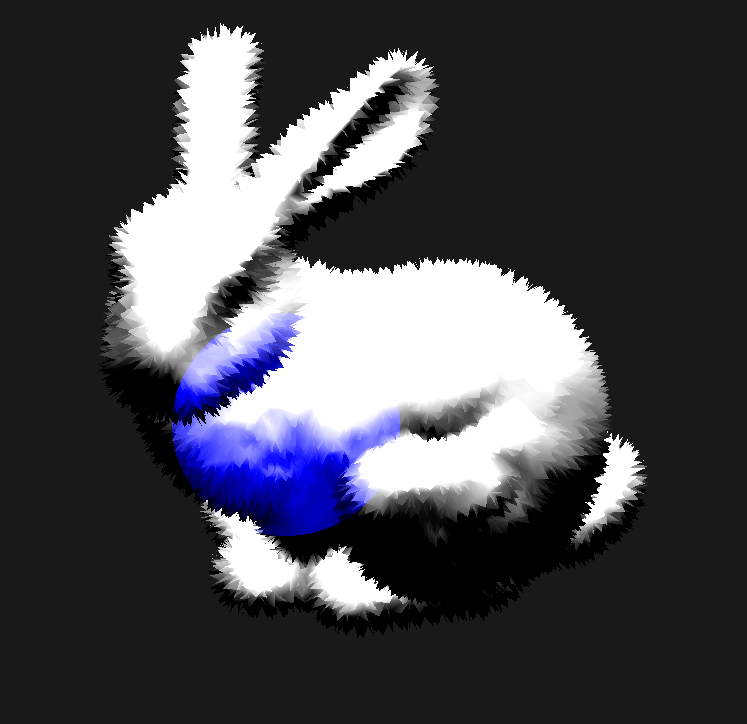
\includegraphics[width=4cm,height=4cm]{final_bunny}
\caption{the final result of bunny}
\end{figure}

\end{document}
